% Конкретные численные значения, которые использовались (входные данные)
\subsection*{Исходные данные экспериментальной модели}
В целях исследования безотказности работы сформированной модели и сложности ее анализа различными решателями проводился ряд экспериментов. В качестве входных данных для разных решателей использовалась одна и та же модель, имеющая такое число ограничений и параметров, которое бы позволило применять решатели по открытой лицензии.
Характеристики оборудования, используемого для проведения экспериментов:
\begin{itemize}
  \item операционная система - Ubuntu 23.04;
  \item процессор - 2-ядерный процессор Intel Core i5 с тактовой частотой 1,8GHz;
  \item объем ОЗУ - 8 ГБ.
\end{itemize}

Размеры матриц входных данных модели своими размерностями удовлетворяют следующим характеристикам задачи:
\begin{center}
  $l = 1, n = 5, m = 4, k = 3$
\end{center}

В экспериментах использовалась модель, построенная на следующих числовых значениях элементов матриц:
\begin{center}
  $
  T = 
  \begin{pmatrix}
      1 &   0 &   0 & 0   \\
    0.5 & 0.5 &   0 & 0   \\
      0 & 0.5 & 0.5 & 0   \\
      0 &   0 & 0.5 & 0.5 \\
      0 &   0 &   0 & 1 
  \end{pmatrix}
  $
\end{center}

\begin{center}
  $
  D = 
  \begin{pmatrix}
    0 & 0 & 0 & 0   \\
    0 & 0 & 1 & 1   \\
    0 & 0 & 0 & 0   \\
    0 & 0 & 0 & 0 
  \end{pmatrix}
  $
\end{center}

\begin{center}
  $
  P = 
  \begin{pmatrix}
    1 & 1 & 1 & 1 & 1   \\
    1 & 1 & 1 & 1 & 1   \\
    1 & 1 & 1 & 1 & 1   \\
    1 & 1 & 1 & 1 & 1   \\
    1 & 1 & 1 & 1 & 1 
  \end{pmatrix}
  $
\end{center}

\begin{center}
  $
  E = \begin{pmatrix}
    1 & 0 & 0 & 0 & 0
  \end{pmatrix}
  $
\end{center}

% Рисунок (граф со стрелками и связями) модели, которую обсчитываем

Представление в виде графа, построенного в соответствии с описанными выше исходными данными модели, изображено на рисунке \ref{fig:graph}.

\begin{figure}[H]
  \centering
  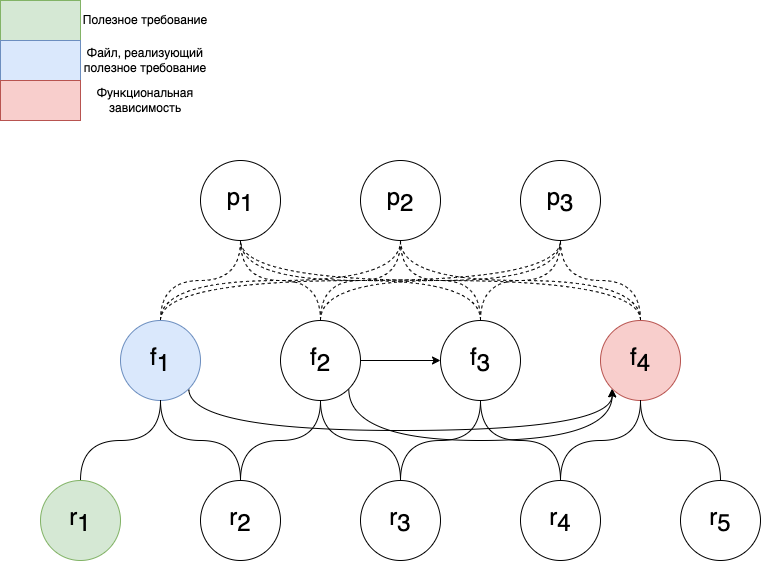
\includegraphics[width=0.8\textwidth]{graph}
  \caption{Предствление в виде графа}
  \label{fig:graph}
\end{figure}

% Информация из принта модели с указанием общего числа параметров модели и ее ограничений

Результирующая математическая модель включает $71$ ограничение и $37$ параметров. Из них $12$ являются искомыми значениями, а $25$ дополнительными параметрами.

% Таблица с применением решателей для решения моей сформированной модели
\subsection*{Результаты экспериментов}
Экспериментальная модель была обсчитана рядом решателей: \textit{glpk}, \textit{gurobi}, \textit{xpress}, \textit{gams}, \textit{gdpopt}, \textit{mindtpy}, \textit{cbc}, \textit{conopt}, \textit{copt}, \textit{cplex}, \textit{ilogcp}, \textit{loqo} и \textit{minos}.

В рамках проведения экспериментов каждый решатель обсчитал модель по $100$ раз. При каждом обсчете замерялось время, необходимое решателю для выполнения вычислений, а так же результирующее значение целевой функции. Каждый из решателей в своей серии экспериментов демонстрировал одинаковое значение целевой функции.

На рисунке \ref{fig:solution} приведены данные о затраченном времени работы каждого из решателей в серии экспериментов, а так же информация о результирующей стоимости.

\begin{figure}[H]
  \centering
  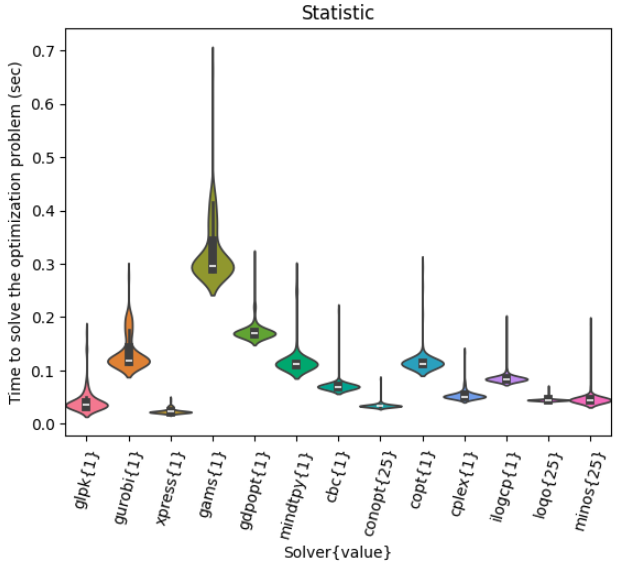
\includegraphics[width=0.8\textwidth]{solution}
  \caption{Результаты экспериментов}
  \label{fig:solution}
\end{figure}

\subsection*{Анализ результатов экспериментов}
Результаты экспериментов показывают, что время, потребное различным решателям для вычисления одних и тех же параметров может отличаться в разы. А так же, что нельзя идентифицировать полученный ответ от решателя как единственно верный. Лучше проводить серию экспериментов с разными решателями для получения достоверного результата.

Наименьшее значение целевой функции, которое было достигнуто решателями, составляет $1$. Это значение было достигнуто $10$-ю решателями из $13$. А наибольшее значение целевой функции составляет $25$ и оно получилось в результате работы $3$-х решателей: \textit{conopt}, \textit{loqo} и \textit{minos}. Наименьшее медианное время, потребное для вычислений, показали решатели \textit{glpk}, \textit{xpress} и \textit{conopt}. Наибольшее время потребовалось решателю \textit{gams}.
